% !TEX root = ../../CompVis.tex
\section{Gegnerating Images}
Idea: Given training samples (images, no labels) generate new samples from the same distribution

\subsection{Approaches}
\begin{minipage}{0.5\textwidth}
    \begin{itemize}
        \item We want to learn a distribution $p_\text{model}(x)$ that is similar to $p_\text{data}$
        \item Explicit density estimation: solve for $p_\text{model}(x)$
        \item Implicit: learn model that can sample from $p_\text{model}(x)$
    \end{itemize}
\end{minipage}
\begin{minipage}{0.5\textwidth}
    \centering
    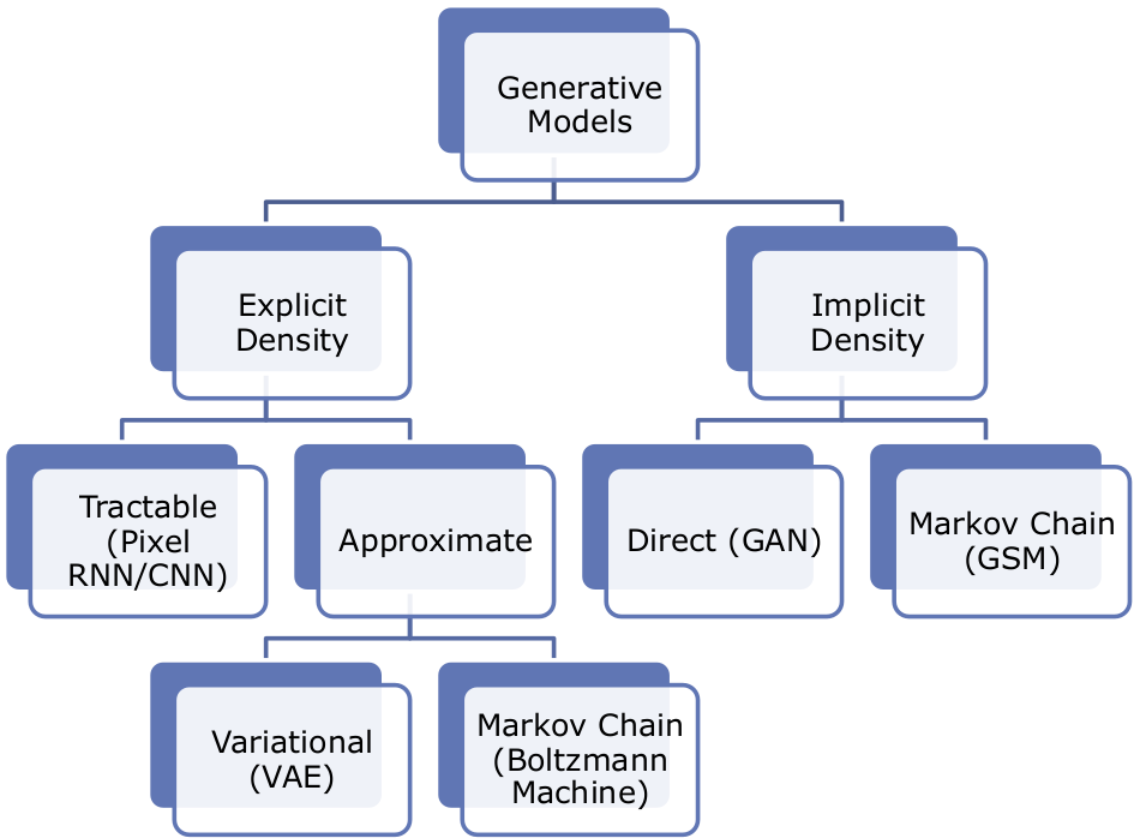
\includegraphics[width=0.9\textwidth]{sections/GeneratingImages/img/taxonomy.png}
\end{minipage}

\subsubsection{Pixel RNN / CNN}
\begin{minipage}{0.5\textwidth}
    \begin{itemize}
        \item Explicit Density Model
        \item Model likelihood of images as dependency to previous pixel values $p(x) = \prod_{i=1}^n p(x_i|x_1,\ldots,x_{i-1})$
        \item Train to minimize the likelihood of the training data
        \item Generate images starting from a corner
        \item RNN: Model dependency on previous pixels using a recurrent neural network (LSTM)
        \item CNN: Model dependency on previous pixels as a CNN over a region
    \end{itemize}
    Pros / Cons
    \begin{itemize}
        \item Can explicitely model the likelihood $p(x)$
        \item Good samples
        \item High resolution images
        \item Long generation time
    \end{itemize}
\end{minipage}
\begin{minipage}{0.5\textwidth}
    \centering
    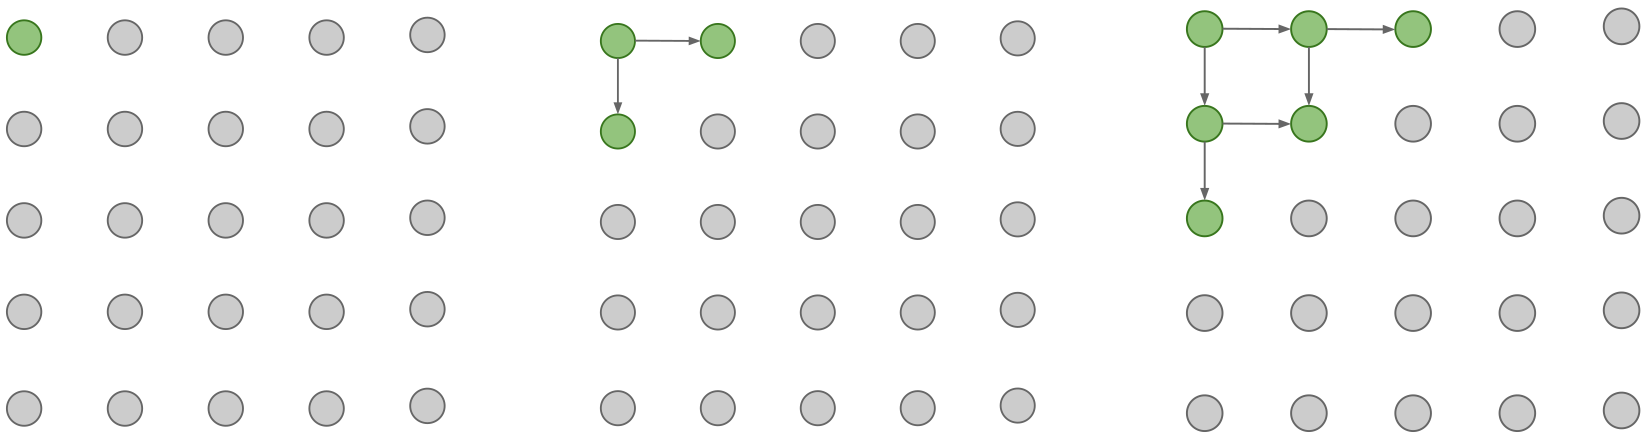
\includegraphics[width=.95\textwidth]{sections/GeneratingImages/img/pixel_rnn.png}

    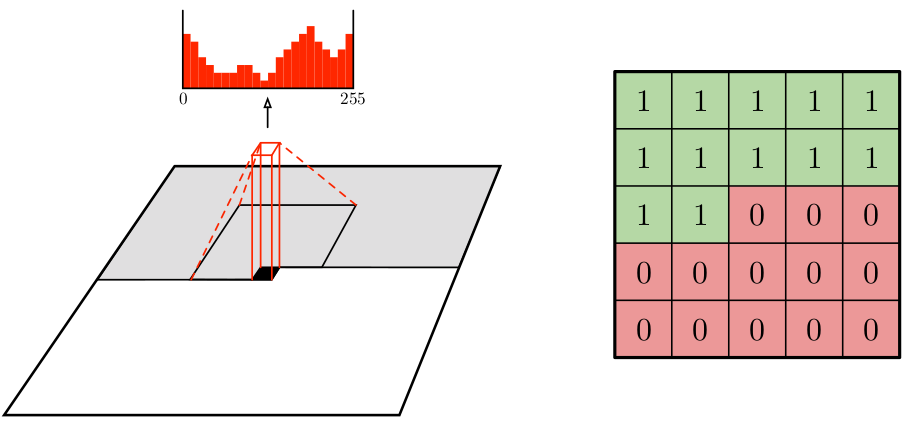
\includegraphics[width=0.9\textwidth]{sections/GeneratingImages/img/pixel_cnn.png}
\end{minipage}

\begin{minipage}{0.8\textwidth}
    \subsubsection{Autoencoders}
    Learns a good feature representation of the data
    \begin{itemize}
        \item Decoder
              \begin{itemize}
                  \item Linear with sigmoid
                  \item Upscaling CNNS
              \end{itemize}
        \item $z$ smaller than $x$: dimensionalty reduction
        \item Encoder
              \begin{itemize}
                  \item Linear with non linearity (sigmoid)
                  \item CNNs with ReLU
              \end{itemize}
        \item Loss $\lVert x - x'\rVert^2$
    \end{itemize}
    Problem: Representations of the (latent) variables $z$ might not be easily interpolated and might have gaps
\end{minipage}
\begin{minipage}{0.2\textwidth}
    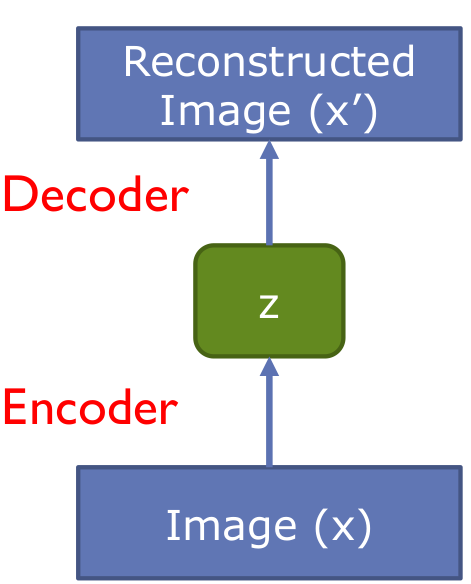
\includegraphics[width=1\textwidth]{sections/GeneratingImages/img/autoencoder.png}
\end{minipage}

\begin{minipage}{0.8\textwidth}
    \subsubsection{Variational Autoencoders}
    Models pixel distribution from a latent variable space $p(x)=\int p(x|z)p(z)dz$
    \begin{itemize}
        \item Choose $p(z)$ to be simple (for example Gaussian)
        \item $p(x|z)$ is complex $\rightarrow$ Model with neural network
        \item The integral hard to calculate $z$ $\rightarrow$ Define network $q(z|x)$ that approximates $p(z|x)$
    \end{itemize}
    Pros/Cons
    \begin{itemize}
        \item Principled approach to generative models
        \item Allows inference of $p(z|x)$ which can be useful for other taskks
        \item Calculation only maximizes lower bound, not as good as in evalution of Pixel RNN/CNN
        \item Samples are blurrier and lower quality than GANs
    \end{itemize}
\end{minipage}
\begin{minipage}{0.2\textwidth}
    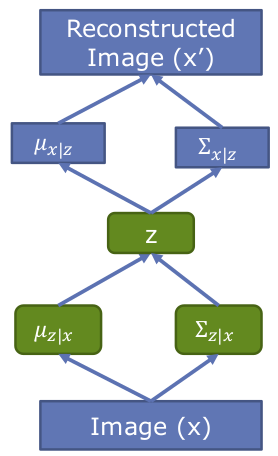
\includegraphics[width=1\textwidth]{sections/GeneratingImages/img/vae.png}
\end{minipage}

\paragraph{Math}
\begin{align*}
    \log p_\theta(x^{(i)}) & = \mathrm{E}_{z \sim q_\phi(z|x^{(i)})}\left[ \log p_\theta(x^{(i)})\right] \qquad (p_\theta(x^{(i)}) \text{ Does not depend on }z )                                                                                                           \\
                           & = \mathrm{E}_{z}\left[ \log \frac{p_\theta(x^{(i)}|z) p_\theta(z)}{p_\theta(z | x^{(i)})} \frac{q_\phi(z|x^{(i)})}{q_\phi(z|x^{(i)})}\right]\qquad \text{(Bayes' Rule and Multiply by constant)}                                               \\
                           & = \mathrm{E}_{z}\left[ \log p_\theta(x^{(i)}|z)\right] - \mathrm{E}_{z}\left[ \log \frac{q_\phi(z|x^{(i)})}{p_\theta(z)} \right] + \mathrm{E}_{z}\left[ \log \frac{q_\phi(z|x^{(i)})}{p_\theta(z| x^{(i)})} \right] \qquad \text{(Logarithms)} \\
                           & = \mathrm{E}_{z}\left[ \log p_\theta(x^{(i)}|z)\right] - D_{KL} \left(q_\phi(z|x^{(i)})\lVert p_\theta(z) \right) + D_{KL}\left(q_\phi(z|x^{(i)})\lVert p_\theta(z| x^{(i)}) \right)
\end{align*}
Still intractable, but it is possible to calculate a lower bound

\subsubsection{Generative Adversial Networks (GAN)}
Make generating images a two person game (generator and discriminator)
\begin{description}
    \item[Generator:] Generate real looking images that fool the discriminator
    \item[Discriminator:] Try to distinguish between real and generated images
\end{description}

\paragraph{Training}
\begin{minipage}{0.5\textwidth}
    Train both networks jointly in a MinMax game: \\$\min_G\max_D V(D,G) = \mathrm{E}_{x \sim p_\text{data}(x)}[\log D(x)] + \mathrm{E}_{z \sim p_z(z)}[\log(1-D(G(z)))]$

    \begin{itemize}
        \item Discriminator ($D$) wants to maximize objective such that $D(x)$ is close to 1 (real) and $D(G(z))$ is close to 0 (fake)
        \item Generator ($G$) wants to minimize objective such that $D(G(z))$ is close to 1 (discriminator is fooled by generated images)
    \end{itemize}
\end{minipage}
\begin{minipage}{0.5\textwidth}
    Best practices
    \begin{itemize}
        \item In practise $\log(1-D(G(z)))$ saturates early in the training when $G$ is poor
        \item It is better to maximise $\log(D(G(z)))$, i.e. instead of minimizing the likelihood of the discriminator to being correct we maximize it to being wrong
        \item Training min max is difficult (essentially you try to find a saddle point on the surface)
        \item New algorithms using Wasserstein GAN
    \end{itemize}
\end{minipage}
\textbf{Algorithm}
\begin{enumerate}
    \item for number of training iterations do
          \begin{enumerate}
              \item for $k$ steps do
                    \begin{enumerate}
                        \item Sample minibatch of $m$ noise samples $\{z^{(1)},\ldots,z^{(m)}\}$ from noise prior $p_g(z)$.
                        \item Sample minibatch of $m$ noise samples $\{z^{(1)},\ldots,z^{(m)}\}$ from data generating distribution $p_\text{data}(x)$.
                        \item Update the discriminator by ascending its stochastic gradient:\newline $\nabla_{\theta_d} \frac{1}{m} \sum_{i=1}^m \left[\log D(x^{(i)}) + \log(1-D(G(z^{(i)})))\right]$
                    \end{enumerate}
              \item Sample minibatch of $m$ noise samples $\{z^{(1)},\ldots,z^{(m)}\}$ from noise prior $p_g(z)$.
              \item Update the generator by descending its stochastic gradient: $\nabla_{\theta_g} \frac{1}{m} \sum_{i=1}^m \log(1-D(G(z^{(i)})))$
          \end{enumerate}
\end{enumerate}

\subsection{Image to Image Transfer}
\begin{minipage}{0.5\textwidth}
    Conditional GAN: Learn mapping from input image $x$ and noise $z$ to output image $y$: $G: \{x,z\} \mapsto y$.
    In practice adding noise as input proves ineffective, as the network learns to ignore it $\rightarrow$ Use dropout as noise
    \begin{itemize}
        \item Training a conditional GAN for image to image transfer to generate an image out of a edge map
        \item In comparison to GANs, in conditional GANs both the Generator and the Discriminator input the edge map
        \item U-Net architectures with connections between the layers seem to work better
    \end{itemize}
\end{minipage}
\begin{minipage}{0.5\textwidth}
    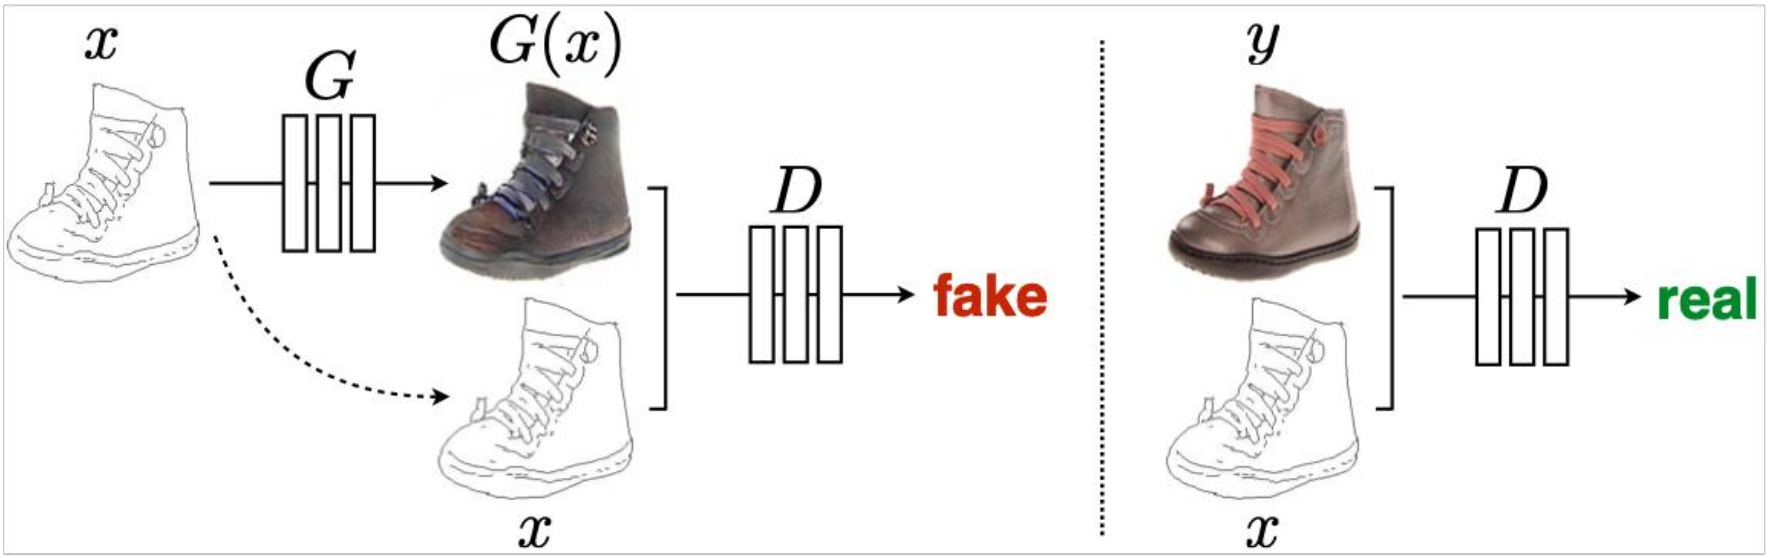
\includegraphics[width=1\textwidth]{sections/GeneratingImages/img/cond_gan.png}
\end{minipage}


\subsection{Visualization of Neural Networks}
\begin{itemize}
    \item First layer(s): Visualize filters directly
    \item Intermediate layers: Apply netowrks to image and visualize activations
    \item Last layer: Feature vector comparison before logits and softmax
    \item Occlusions: Mask part of image and check how much the predicted probabilities change
\end{itemize}

\subsubsection{Deep Dream}
\begin{minipage}{0.5\textwidth}
    Idea: Amplify the activations at some layers in the network

    Select image and layer in a CNN
    \begin{enumerate}
        \item Forward computation of activations at chosen layer
        \item Set gradient of layer equal to its activation
        \item Backward: Propagate to compute gradient on image
        \item Update image
    \end{enumerate}
\end{minipage}
\begin{minipage}{0.5\textwidth}
    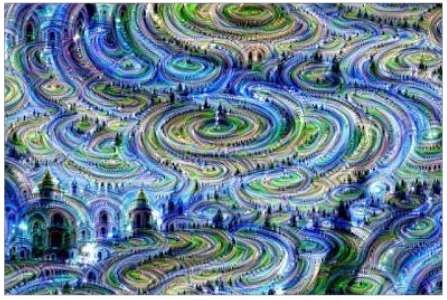
\includegraphics[width=0.5\textwidth]{sections/GeneratingImages/img/deepdream1.png}
    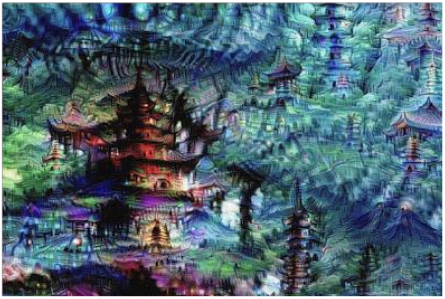
\includegraphics[width=0.49\textwidth]{sections/GeneratingImages/img/deepdream2.png}
\end{minipage}

\subsection{Texture Synthesis}
Two main approaches: Replicate pixels and patches using a suitable algorithm or find a model (CNN) of the texture and generate new textures from the model

\begin{minipage}{0.4\textwidth}
    Synthesis:
    \begin{enumerate}
        \item Pass image $x$ through the network (VGG net)
        \item The activations from each layer are feature maps $F^l \in \mathbb{R}^{N\times M}$ for the texture
        \item Calculate Gram matrix to compute correlations between feature maps (on the same layers) $G_{ij}^l = \sum_k F_{ik}^l F_{jk}^l$
    \end{enumerate}
    Generating:
    \begin{enumerate}
        \item Start with noise image
        \item Use gradient descent to find another image that matches the Gram-matrix representation of the original image
        \item Optimize by minimizing the mean-squared distance between the matrices from the original and generated image
        \item Use standard forward / backward computations of the network
    \end{enumerate}
\end{minipage}
\begin{minipage}{0.6\textwidth}
    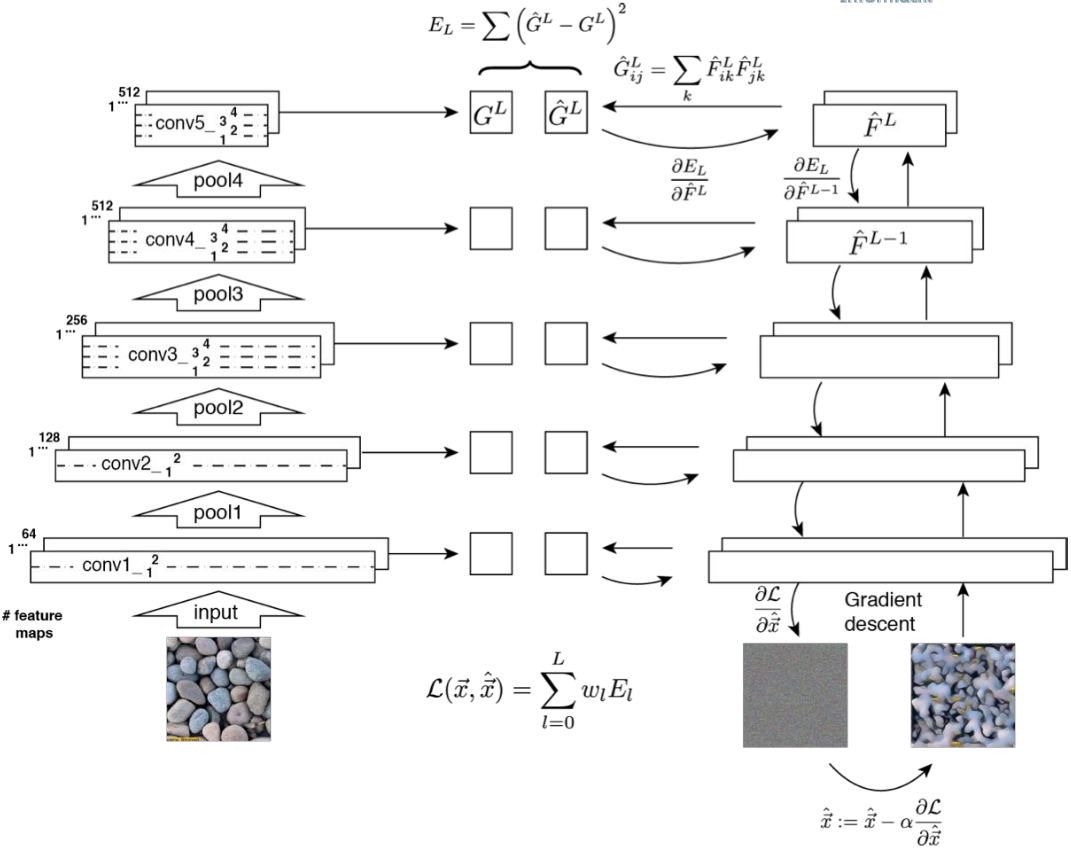
\includegraphics[width=\textwidth]{sections/GeneratingImages/img/generate_textures.png}
\end{minipage}

\subsection{Style Transfer}
\begin{minipage}{0.5\textwidth}
    Content representation
    \begin{itemize}
        \item Each input image generates filter response \newline $F^l \in \mathbb{R}^{N \times M}$ at each layer
        \item We can run gradient descend on noise images to find an image that generates the same response
        \item If $F^l \in \mathbb{R}^{N \times M}$ is the response from the original image and $P^l \in \mathbb{R}^{N \times M}$ the response from the generated image, the loss is $\mathcal{L}_\text{content}=(p,x,l)=\frac{1}{2}\sum_{i,j}\left(F_{ij}^l + P_{ij}^l\right)^2$
        \item Later loss in the network define the content
    \end{itemize}
\end{minipage}
\begin{minipage}{0.5\textwidth}
    Style representation
    \begin{itemize}
        \item Each input image generates filter responses $F^l \in \mathbb{R}^{N \times M}$ at each layer, calculate Gram matrices from the features
        \item If $A^l$ is the matrix from the original image and $G^l$ the matrix from the generated image, the loss for one layer is \newline $E_l = \frac{1}{4N_l^2M_l^2}\sum_i,j \left(G_{ij}^l - A_{ij}^l\right)^2$
        \item and from including several layers \newline $\mathcal{L}_\text{style}(a,x) = \sum_{l=0}^L w_l E_l$
    \end{itemize}
\end{minipage}
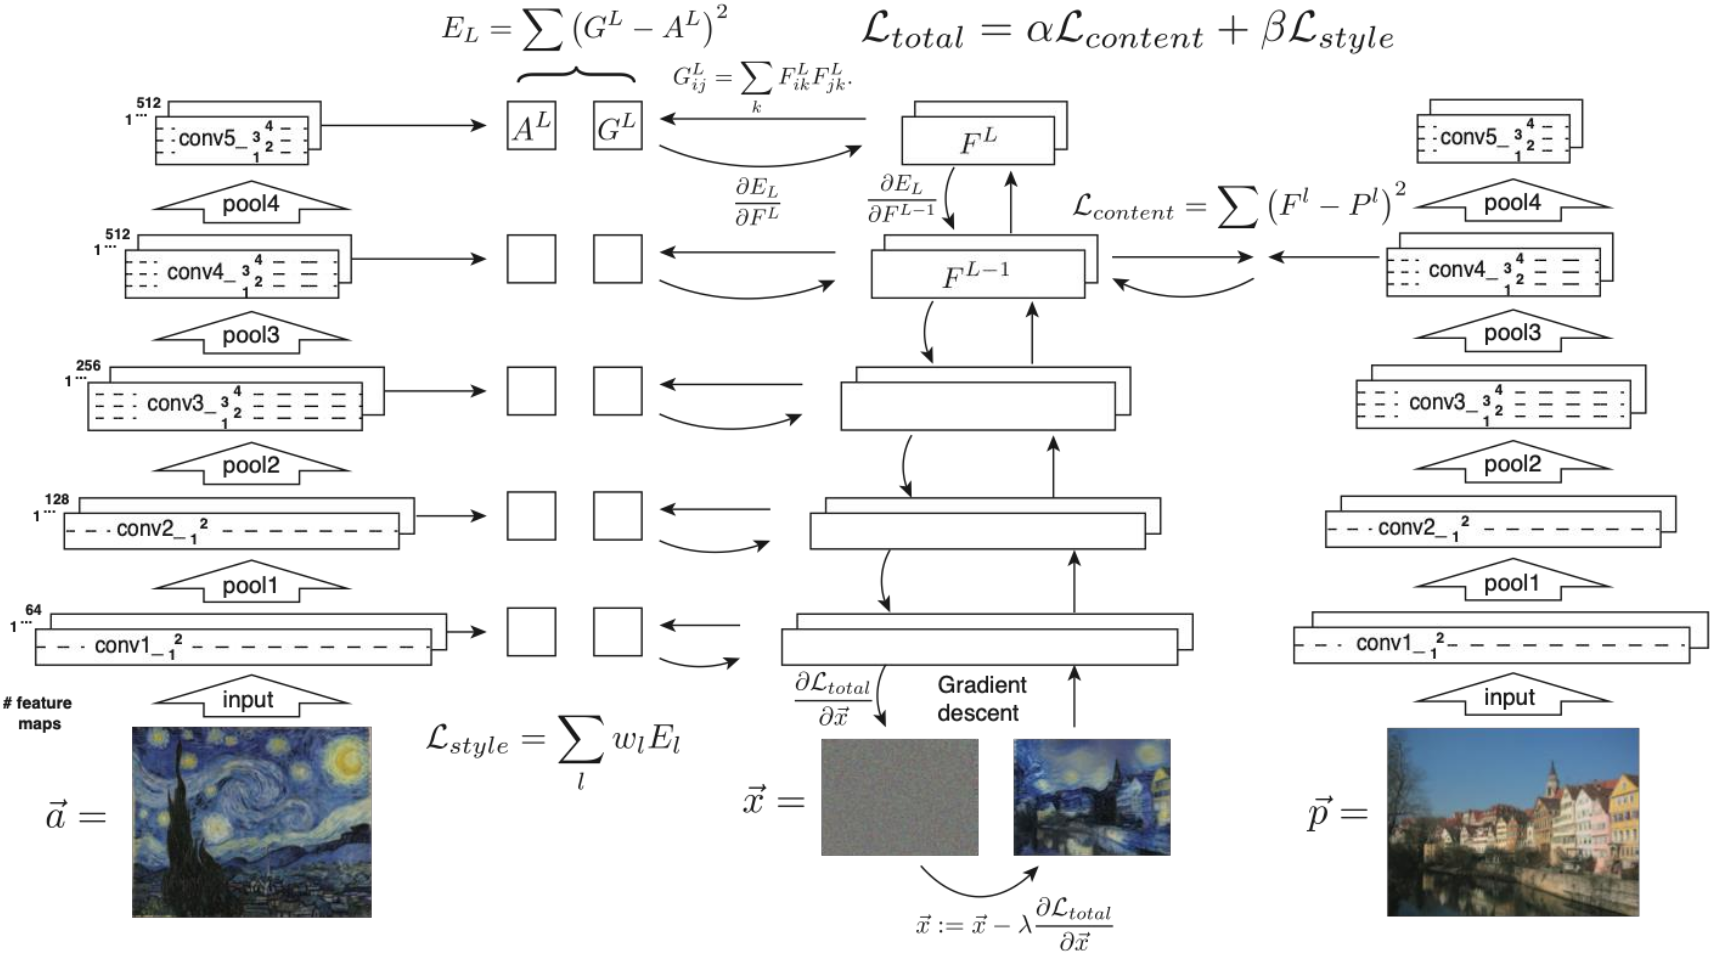
\includegraphics[width=1\textwidth]{sections/GeneratingImages/img/style_transfer.png}

\textbf{Fast Style Transfer:} Train feedforward network for each style and use pretrained CNN with losses as before.
After training, stylize image with single pass forward